\documentclass{beamer}

\author{AJ Fagan}
\title{Network Synergy Recent Papers}
\date{October 4, 2024}

\usepackage{graphicx}
\usepackage{subcaption}
%\graphicspath{ { ./figs } }

\usetheme{Madrid}
\usecolortheme{beaver}




\AtBeginSection[]
{
  \begin{frame}
    \frametitle{Table of Contents}
    \tableofcontents[currentsection]
  \end{frame}
}


%\usepackage[backend=biber, natbib=true]{biblatex}
\bibliographystyle{plain}
%\addbibresource{main.bib}

\begin{document}

\frame{\titlepage}


\begin{frame}
  \frametitle{Table of Contents}
  \tableofcontents 
\end{frame}

\section{Drug Synergy}

\begin{frame}
  \frametitle{Synergy via Potency}
  \begin{figure}[!htb]
      \centering 
      \begin{minipage}[b]{0.49\textwidth}
	\begin{subfigure}[b]{\textwidth}
	  \centering
	  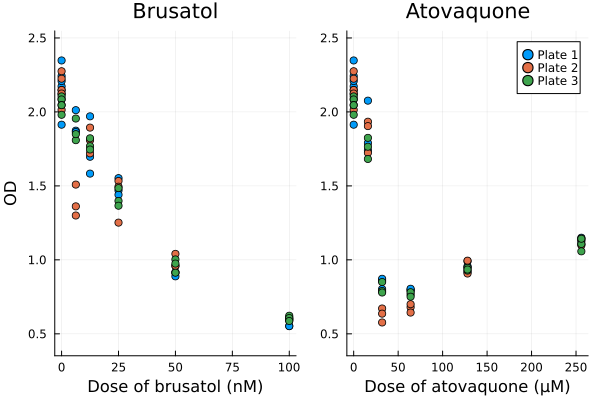
\includegraphics[width=\linewidth]{figs/mono-dose-resp.png}
	\end{subfigure}\vfill
	\begin{subfigure}[c]{\textwidth}
	  \centering
	  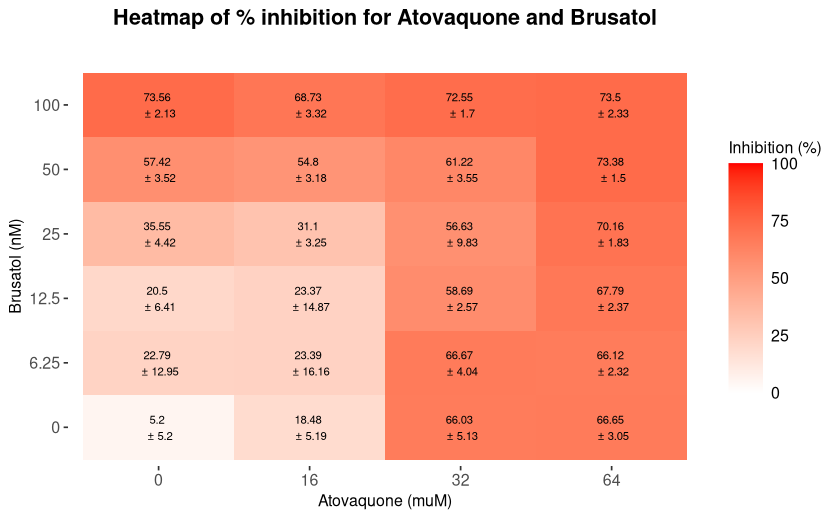
\includegraphics[width=\linewidth]{figs/ato-bru-resp-heatmap.png}
	\end{subfigure}
      \end{minipage}\hfill
      \begin{minipage}[b]{0.49\textwidth}
	\vfill
	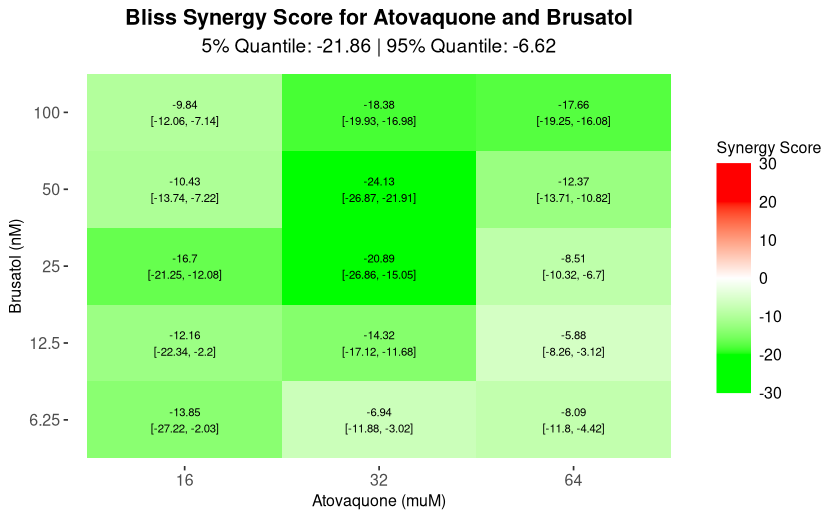
\includegraphics[width=\textwidth]{figs/ato-bru-bliss-heatmap.png}
	\vfill
      \end{minipage}
  \end{figure}
\end{frame}

\begin{frame}
  \frametitle{Promises of Synergistic Combinations}
  The promises associated with synergistic drug combinations are:
  \begin{center}
    \begin{itemize}
      \item Overcoming chemoresistance \only<2>{\checkmark} 
      \item Repurposing existing drugs \only<2>{\checkmark}
      \item Increasing efficacy \only<2>{\checkmark}
      \item \alert<2>{Reducing toxicity}
    \end{itemize}
  \end{center}

\end{frame}

\begin{frame}
  \frametitle{Relevant XKCD}

  \begin{figure}[!htb]
    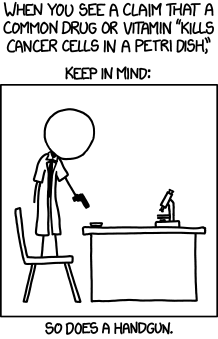
\includegraphics[width=0.4\textwidth]{figs/xkcd-cells.png}
  \end{figure}
\end{frame}

\begin{frame}
  \frametitle{Synergy via Biological Networks}
  Goal: describe the mechanism, rather than the strength, of interaction between two drugs.
  \vfill
  \begin{figure}
    \centering
    \minipage{0.4\textwidth}
      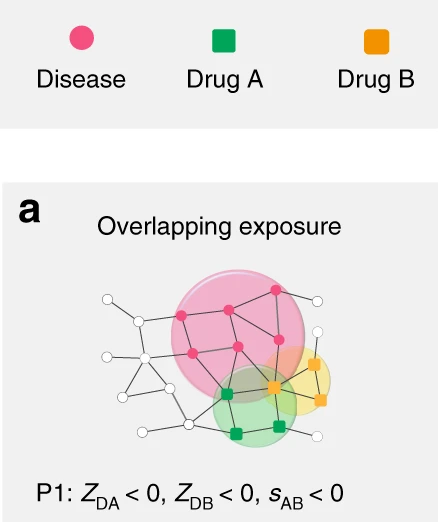
\includegraphics[width=\linewidth]{figs/barabasi-hypertension-overlapping-net.png}
    \endminipage\hfill 
    \minipage{0.59\textwidth}
      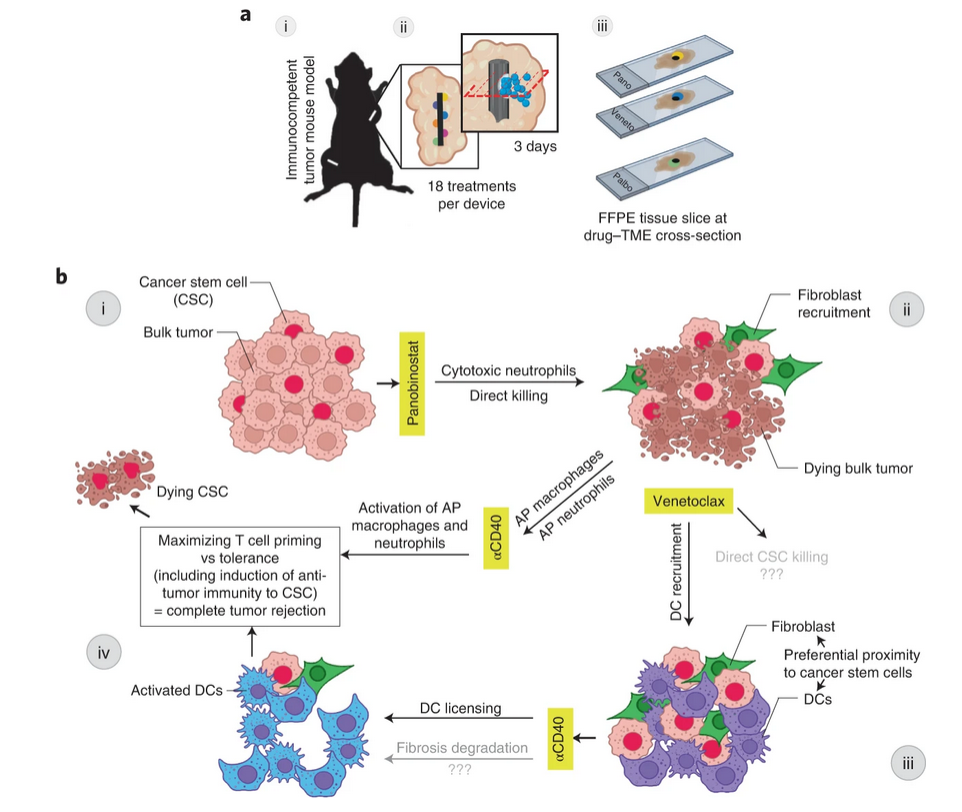
\includegraphics[width=\linewidth]{figs/TME_example.png}
    \endminipage
  \end{figure}
\end{frame}

\section{Network Synergy via Modules}


\begin{frame}
  \frametitle{Module Approach}
  \begin{figure}[!htb]
    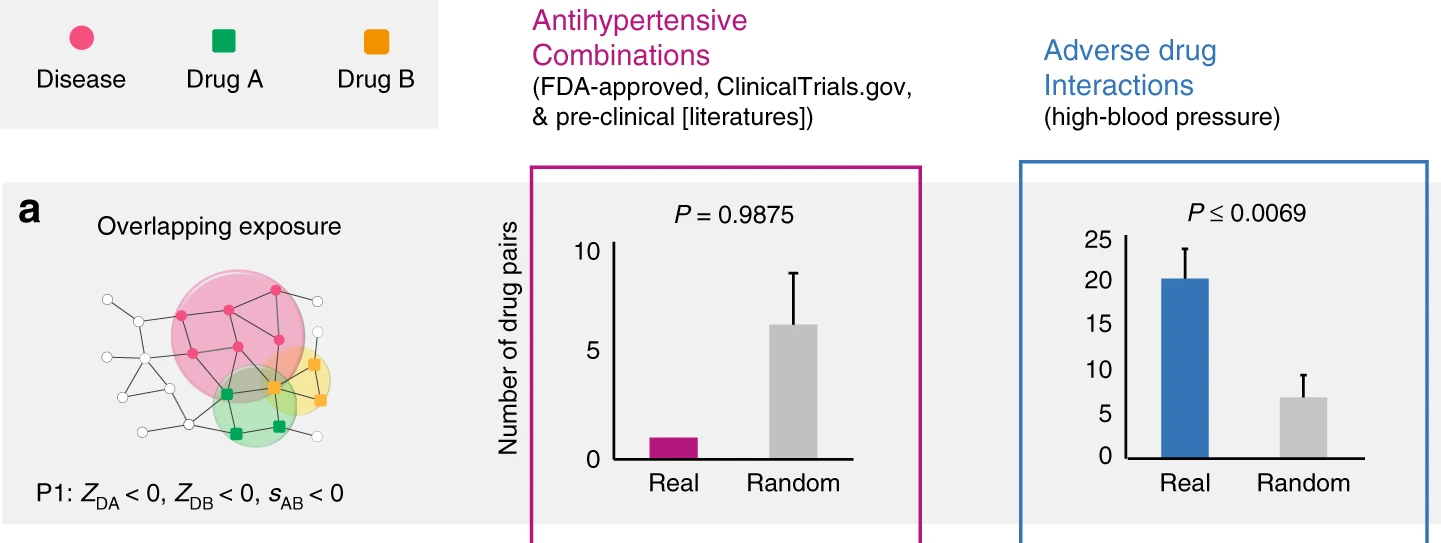
\includegraphics[width=\linewidth]{figs/barabasi-hypertension-overlapping.png}
  \end{figure}
  \small{\textit{Network-based prediction of drug combinations}, Cheng, Kovacs, Barabasi, 2019}~\cite{Cheng2019} 
\end{frame}

\begin{frame}
  \frametitle{Module Approach}
  \begin{figure}[!htb]
    \minipage{0.48\textwidth}
      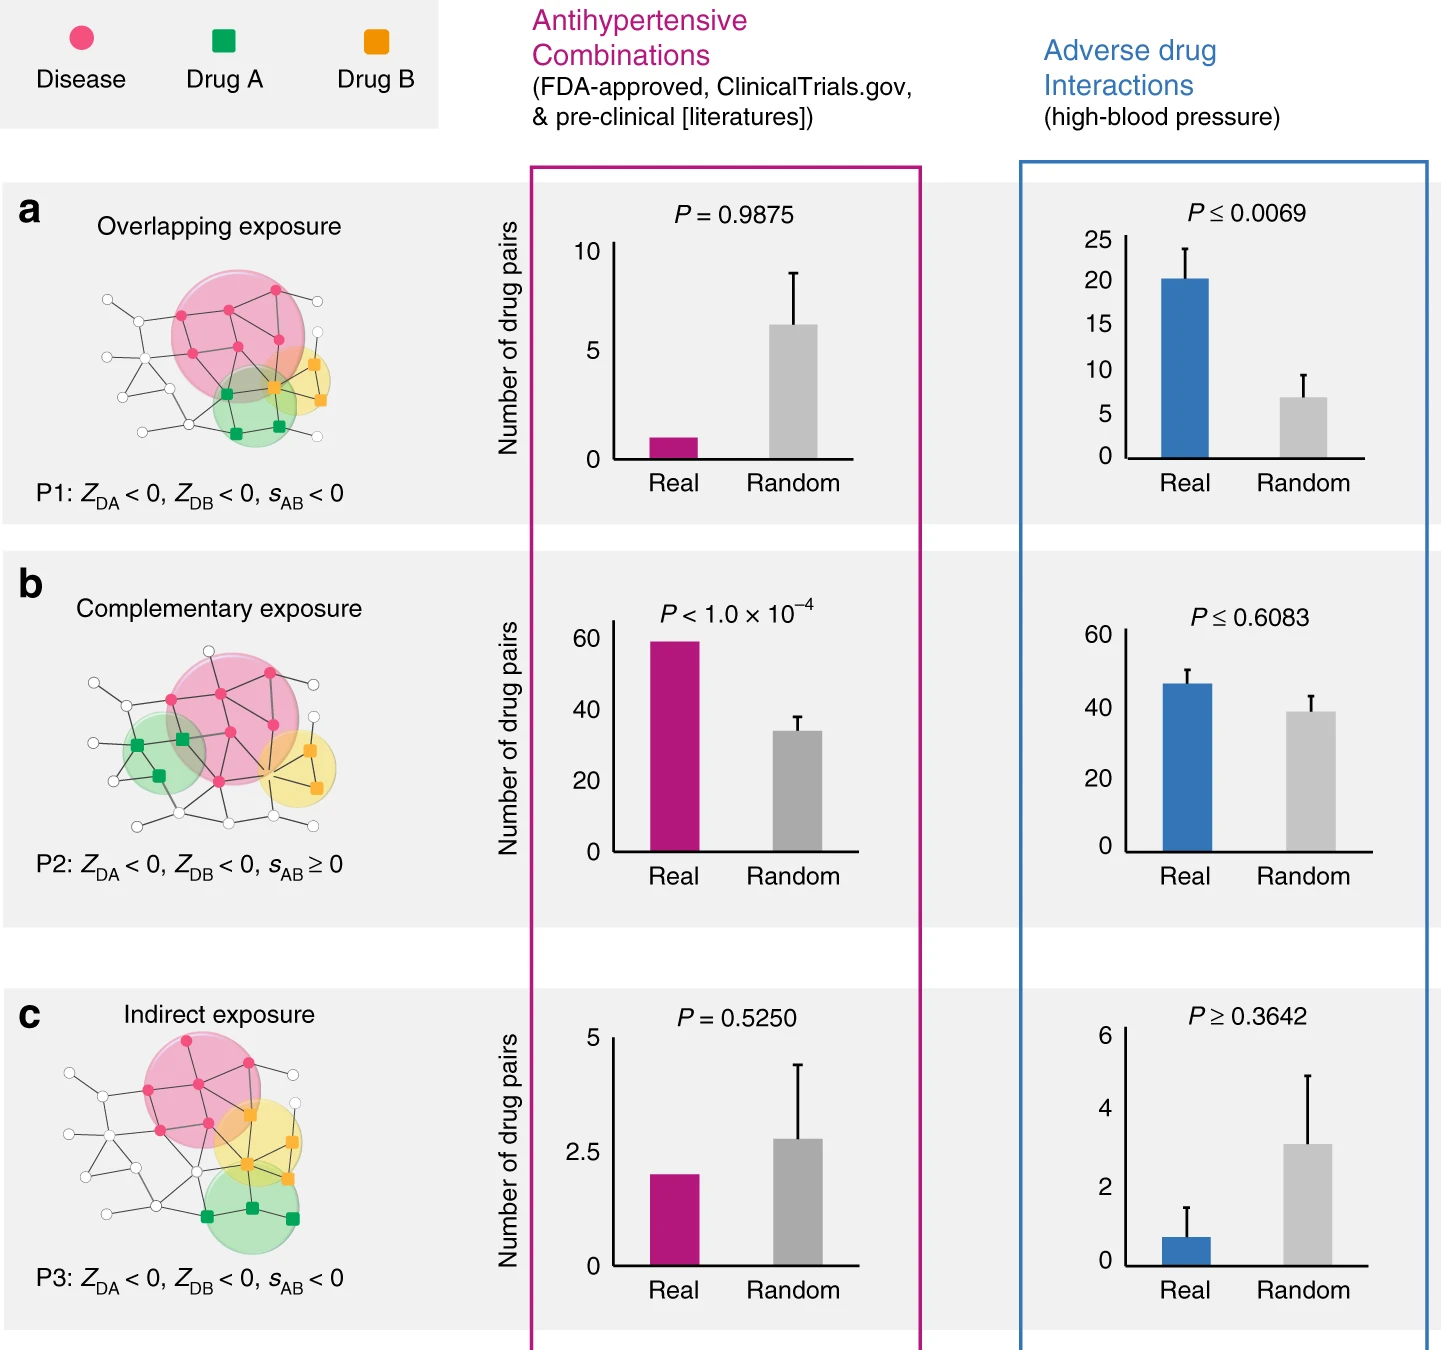
\includegraphics[width=\linewidth]{figs/barabasi-hypertension_a-c.png}
    \endminipage\hfill 
    \minipage{0.48\textwidth}
      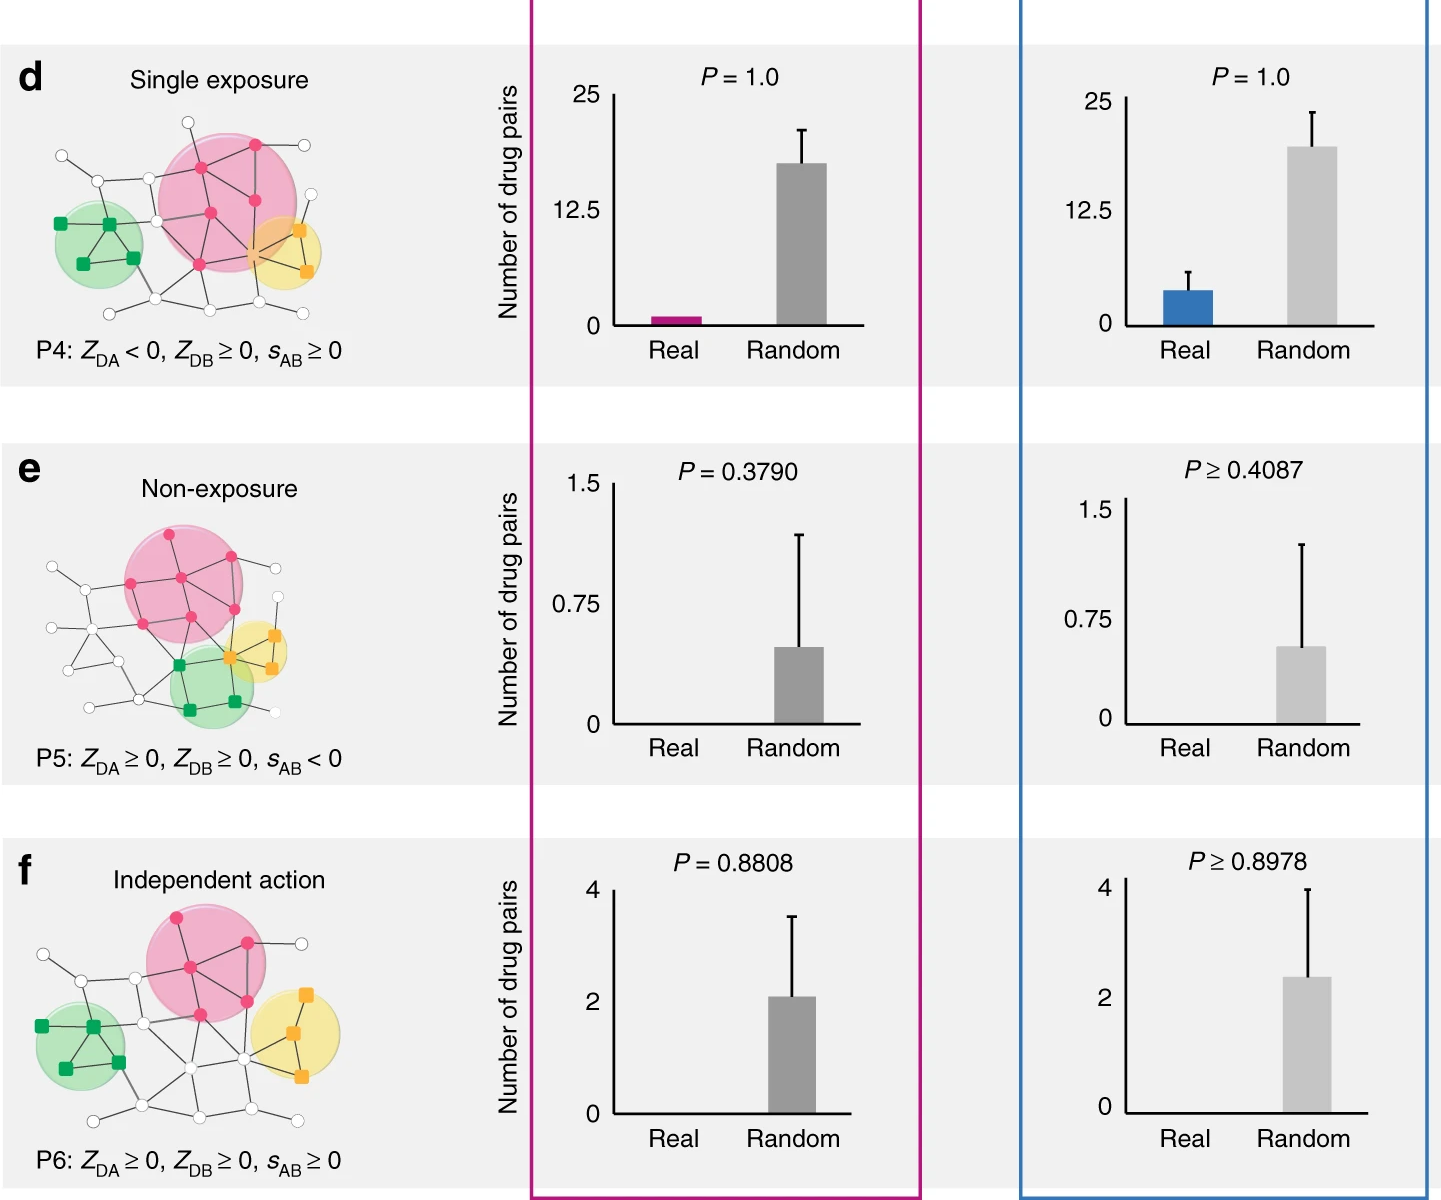
\includegraphics[width=\linewidth]{figs/barabasi-hypertension_d-f.png}
    \endminipage
  \end{figure}
  \small{\textit{Network-based prediction of drug combinations}, Cheng, Kovacs, Barabasi, 2019}~\cite{Cheng2019} 
\end{frame}



\section{Synergy in Transcriptional Profiles}

\begin{frame}
  \frametitle{Synergy in Transcriptional Profiles}
  \begin{figure}[!htb] 
    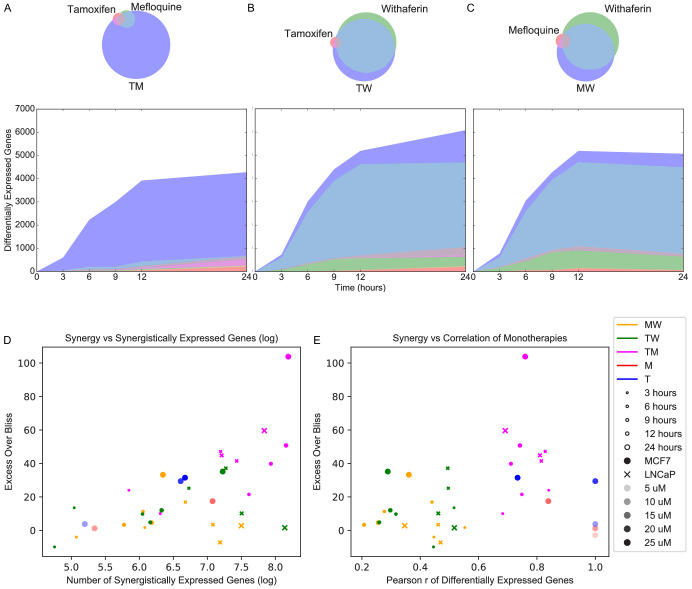
\includegraphics[width=0.6\textwidth]{figs/transcriptomic-synergy.jpg}
  \end{figure}
  \small{\textit{The transcriptomic response of cells to a drug combination is more than the sum of the responses to the monotherapies}, Diaz et. al., 2020}~\cite{Diaz2020-bi}
\end{frame}

\begin{frame}
  \frametitle{Synergistically Expressed Genes in GSEA}
  \begin{figure}[!htb]
    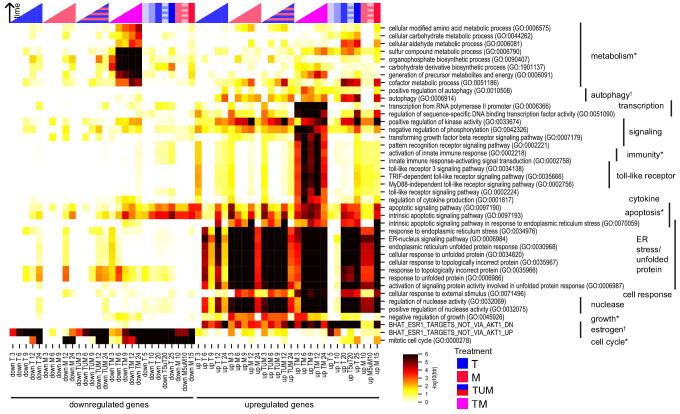
\includegraphics[width=0.8\textwidth]{figs/transcriptomic-synergy-gsea.jpg}
  \end{figure}
  \small{\textit{The transcriptomic response of cells to a drug combination is more than the sum of the responses to the monotherapies}, Diaz et. al., 2020}~\cite{Diaz2020-bi}
\end{frame}

\begin{frame}
  \frametitle{Transcription Cascade of Differentially Active TFs}
  \begin{figure}[!htb]
    \minipage{0.48\textwidth}
      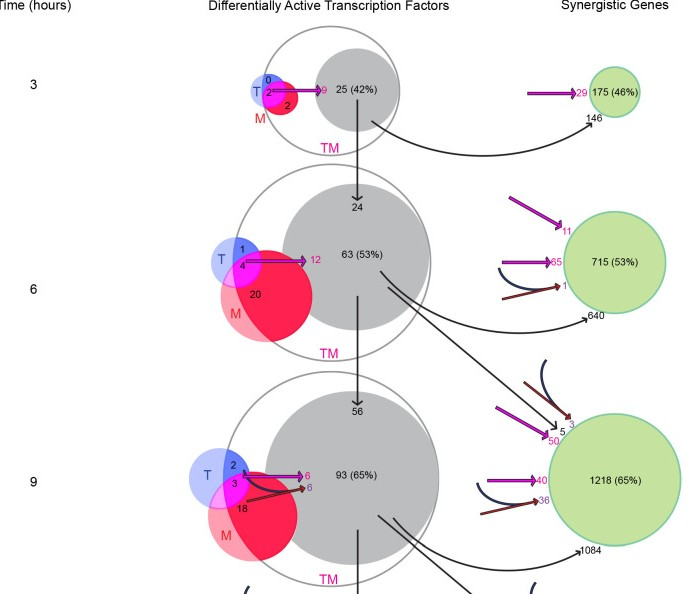
\includegraphics[width=\linewidth]{figs/transcription-cascade_a.jpg}
    \endminipage\hfill 
    \minipage{0.48\textwidth}
      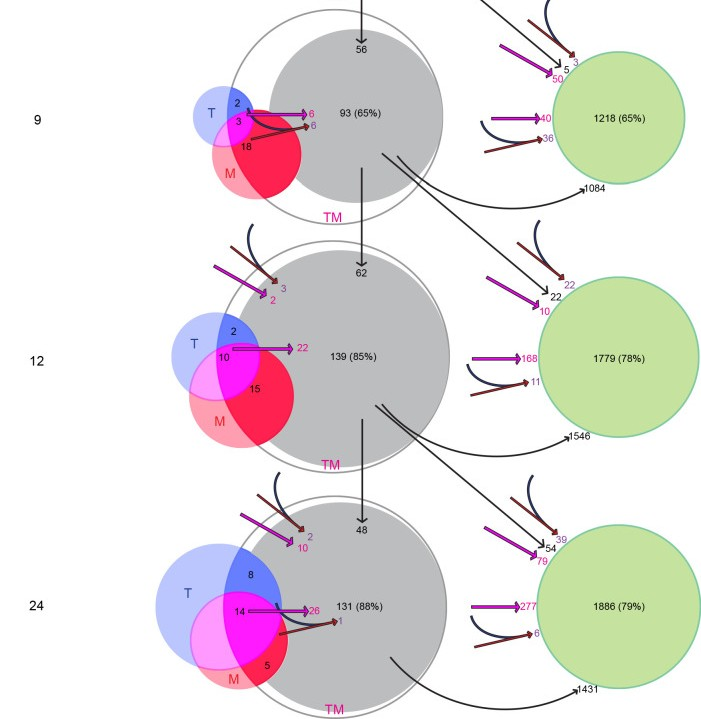
\includegraphics[width=\linewidth]{figs/transcription-cascade_b.jpg}
    \endminipage
  \end{figure}
  \small{\textit{The transcriptomic response of cells to a drug combination is more than the sum of the responses to the monotherapies}, Diaz et. al., 2020}~\cite{Diaz2020-bi}
\end{frame}

\begin{frame}
  \frametitle{The Sham-Combination Principle}
  \begin{block}{The Sham-Combination Principle} 
    A drug combined with itself should be additive.
  \end{block}
  \begin{figure}[!htb]
    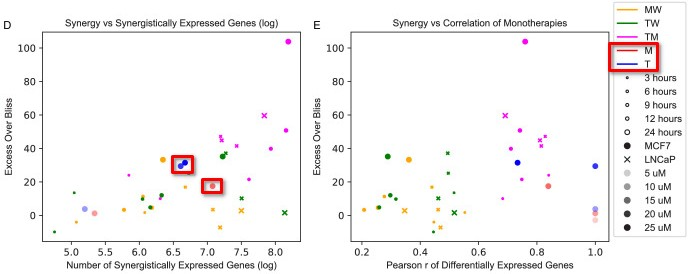
\includegraphics[width=0.8\textwidth]{figs/transcriptomic-synergy-sham_failure.jpg}
  \end{figure}
  \small{\textit{The transcriptomic response of cells to a drug combination is more than the sum of the responses to the monotherapies}, Diaz et. al., 2020}~\cite{Diaz2020-bi}
\end{frame}

\section{Tumor Microenvironments}

\begin{frame}
  \frametitle{Multiplex Implantable Microdevice Assay}
  %\begin{figure}[!htb]
    \minipage{0.43\textwidth}
      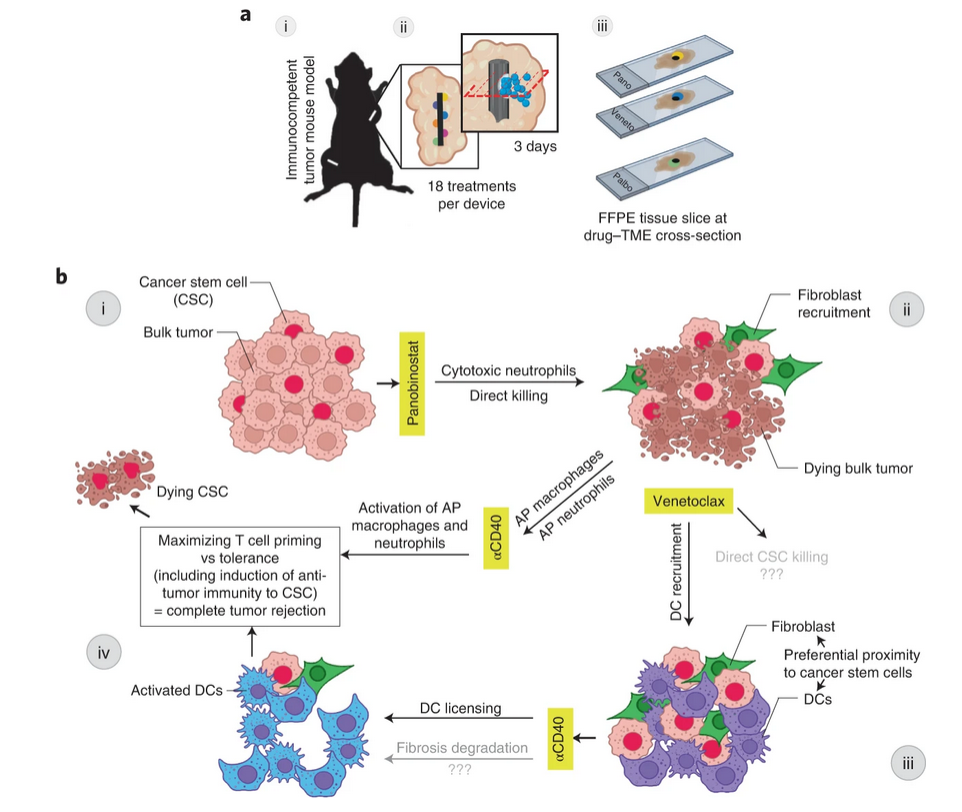
\includegraphics[width=\linewidth]{figs/TME_example.png}
    \endminipage\hfill
    \minipage{0.53\textwidth}
      \begin{itemize}
	\item An Implantable Microdevice (IMD) emits a small amount of several types of drugs into spatially separated regions of the tissue 
	\item Multiplexed Immunohistochemical (mIHC) stainings enable spatial analysis of the TME's response to each treatment 
	\item Synergisic treatment combinations, such as immunotherapies, can be predicted from the results
      \end{itemize}
    \endminipage\vfill
    \small{\textit{Identifying drug combinations that enhance treatment responses mediated by the tumor microenvironment}, Tatarova, Jonas, and Gray, 2022}~\cite{MIMA-Gray-2022}
  %\end{figure}
\end{frame}
 


\section{Available Data}

\begin{frame}
  \frametitle{Available Data}
  \begin{itemize}
    \item Time-course bulk RNA-Seq of Tamoxifin, Withaferin, and Mefloquine in different doses, including pairwise combinations 
    \item Drug targets for 42 drugs, and 73 experimentally verified combinations of them 
    \item Various mIHC and/or cycIF imaging from murine breast cancer models 
    \item \alert{``Combi-seq'' (bulk RNA-seq, but for many drug combinations) data for 420 drug combinations}~\cite{Mathur2022}
  \end{itemize}
\end{frame}

\medskip

\begin{frame}[allowframebreaks]
  \frametitle{References}
  %\printbibliography
  \bibliography{main}
\end{frame}
\end{document}
